% pdf/a 
\begin{filecontents*}[overwrite]{\jobname.xmpdata}
	\Title{Heterogén számítási rendszerek házi feladat dokumentáció}
	\Author{Szilágyi Gábor}
	\Language{hu-HU}
	\Subject{5×5-ös mediánszűrő}
	\Keywords{Mediánszűrő, Batcher odd-even mergesort}
	\Publisher{Szilágyi Gábor}
\end{filecontents*}

\documentclass[a4paper,12pt,titlepage]{article}
%\documentclass[a4paper,12pt,titlepage,draft]{article}
\usepackage{ucs}
\usepackage[T1]{fontenc}
\usepackage[utf8]{inputenc}
\usepackage[magyar]{babel}
\usepackage{amsfonts}
\usepackage{amsmath,bm}
%\usepackage{mathtools} % for \ceil*{}
\usepackage{amssymb}
\usepackage{graphicx}
%\usepackage[hang]{caption}
\usepackage{subcaption}
\usepackage{blkarray,booktabs,bigstrut} % a címkézett mátrixhoz
%\usepackage{enumerate}
%\usepackage{psfrag}
\usepackage[left=25mm,right=25mm,top=25mm,bottom=25mm]{geometry}
%\usepackage[hyphenbreaks]{breakurl}
%\usepackage[hyphens]{url}
%\usepackage{multirow}
%\usepackage{booktabs}
\usepackage{hyperref}
\usepackage{listings}
%\usepackage{cite}
%\usepackage{csquotes}
\usepackage{inconsolata}
\usepackage{siunitx}
\usepackage{xcolor}
\usepackage[a-3u]{pdfx}
\hypersetup{
	colorlinks,
%	 linkcolor={red!50!black},
	linkcolor={black},
%	 citecolor={blue!50!black},
	citecolor={black},
%	 urlcolor={blue!80!black}
	urlcolor={blue!80!black}
}

\definecolor{mygray}{RGB}{240, 240, 240}
\definecolor{mygreen}{RGB}{0, 140, 40}

\sisetup{
	range-phrase=--,
	range-units=single,
	output-decimal-marker={,},
	tight-spacing=true,
	print-unity-mantissa=false,
}

\lstset{ % General setup for the package
	language=C++,
	basicstyle=\scriptsize\ttfamily,
	numbers=left,
	numberstyle=\tiny,
	tabsize=2,
	backgroundcolor=\color{mygray},
	columns=fixed,
	showstringspaces=false,
	showtabs=false,
	keepspaces,
	frame=trbl,
	breaklines=true,
	%breakwhitespace=true,
	morekeywords={sort2,sort8},
	stringstyle=\color{red},
	commentstyle=\color{mygreen},
	keywordstyle=\color{blue}
}

\sloppy % Margón túllógó sorok tiltása.
\widowpenalty=10000 \clubpenalty=10000 %A fattyú- és árvasorok elkerülése
\def\hyph{-\penalty0\hskip0pt\relax} % Kötőjeles szavak elválasztásának engedélyezése

\frenchspacing
\pagestyle{plain} 

%\listfiles % a package-ek kilistázása a logba

\title{
	\centering
	
\includegraphics[width=0.48\textwidth]{kep/bme_logo.pdf} \\
	\vspace{0.5cm}
	\large{\bf Budapesti Műszaki és Gazdaságtudományi Egyetem \\
	Villamosmérnöki és Informatikai Kar \\
	Méréstechnika és Információs Rendszerek Tanszék}\\
	\vspace{5cm}
	\Large{\bf{Heterogén számítási rendszerek\\házi feladat dokumentáció}} \\
	\vspace{3cm}
}

%\parskip=10pt
%\parindent=0pt

\author{Szilágyi Gábor \\ Neptun: NOMK01\\\vspace{1cm}}
\date{Budapest, \today}

\begin{document}
	\maketitle
	\setcounter{page}{2}
	\tableofcontents
	\clearpage
	\section{A használt algoritmus ismertetése}
		A házi feladat egy kép pixelein történő medián szűrés $5\times5$-ös ablakkal, ami 25 elemből a medián kiválasztását jelenti, minden kimeneti pixelhez a három színcsatornára külön-külön.

		A házi feladatomhoz a Batcher odd-even mergesort algoritmust választottam \cite{batcher}. Ez az algoritmus eredeti formájában egy $n=2^k$ elem fölötti rendezés, nem csak mediánkiválasztás, ezzel valamennyi fölösleges része is van, ezt el lehet hagyni az én esetemben. Az algoritmus a rendezendő elemek értékétől független szerkezetű, ezért reprezentálható egy rendezési hálózattal (sorting network). A rendezési hálózat $n=8$ és $n=32$ esetén \aref{fig:batcher-sort}. ábrán látható.

		\begin{figure}[h]
				\centering
				\begin{subfigure}{0.3\textwidth}
					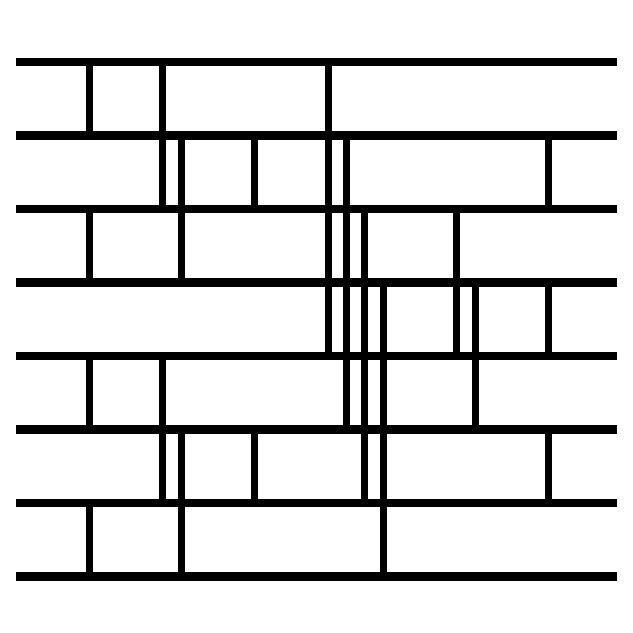
\includegraphics[width=\textwidth]{kep/sort8.eps}
					\caption{$n=8$}
				\end{subfigure}
				\hspace{0.1\textwidth}
				\begin{subfigure}{0.58\textwidth}
					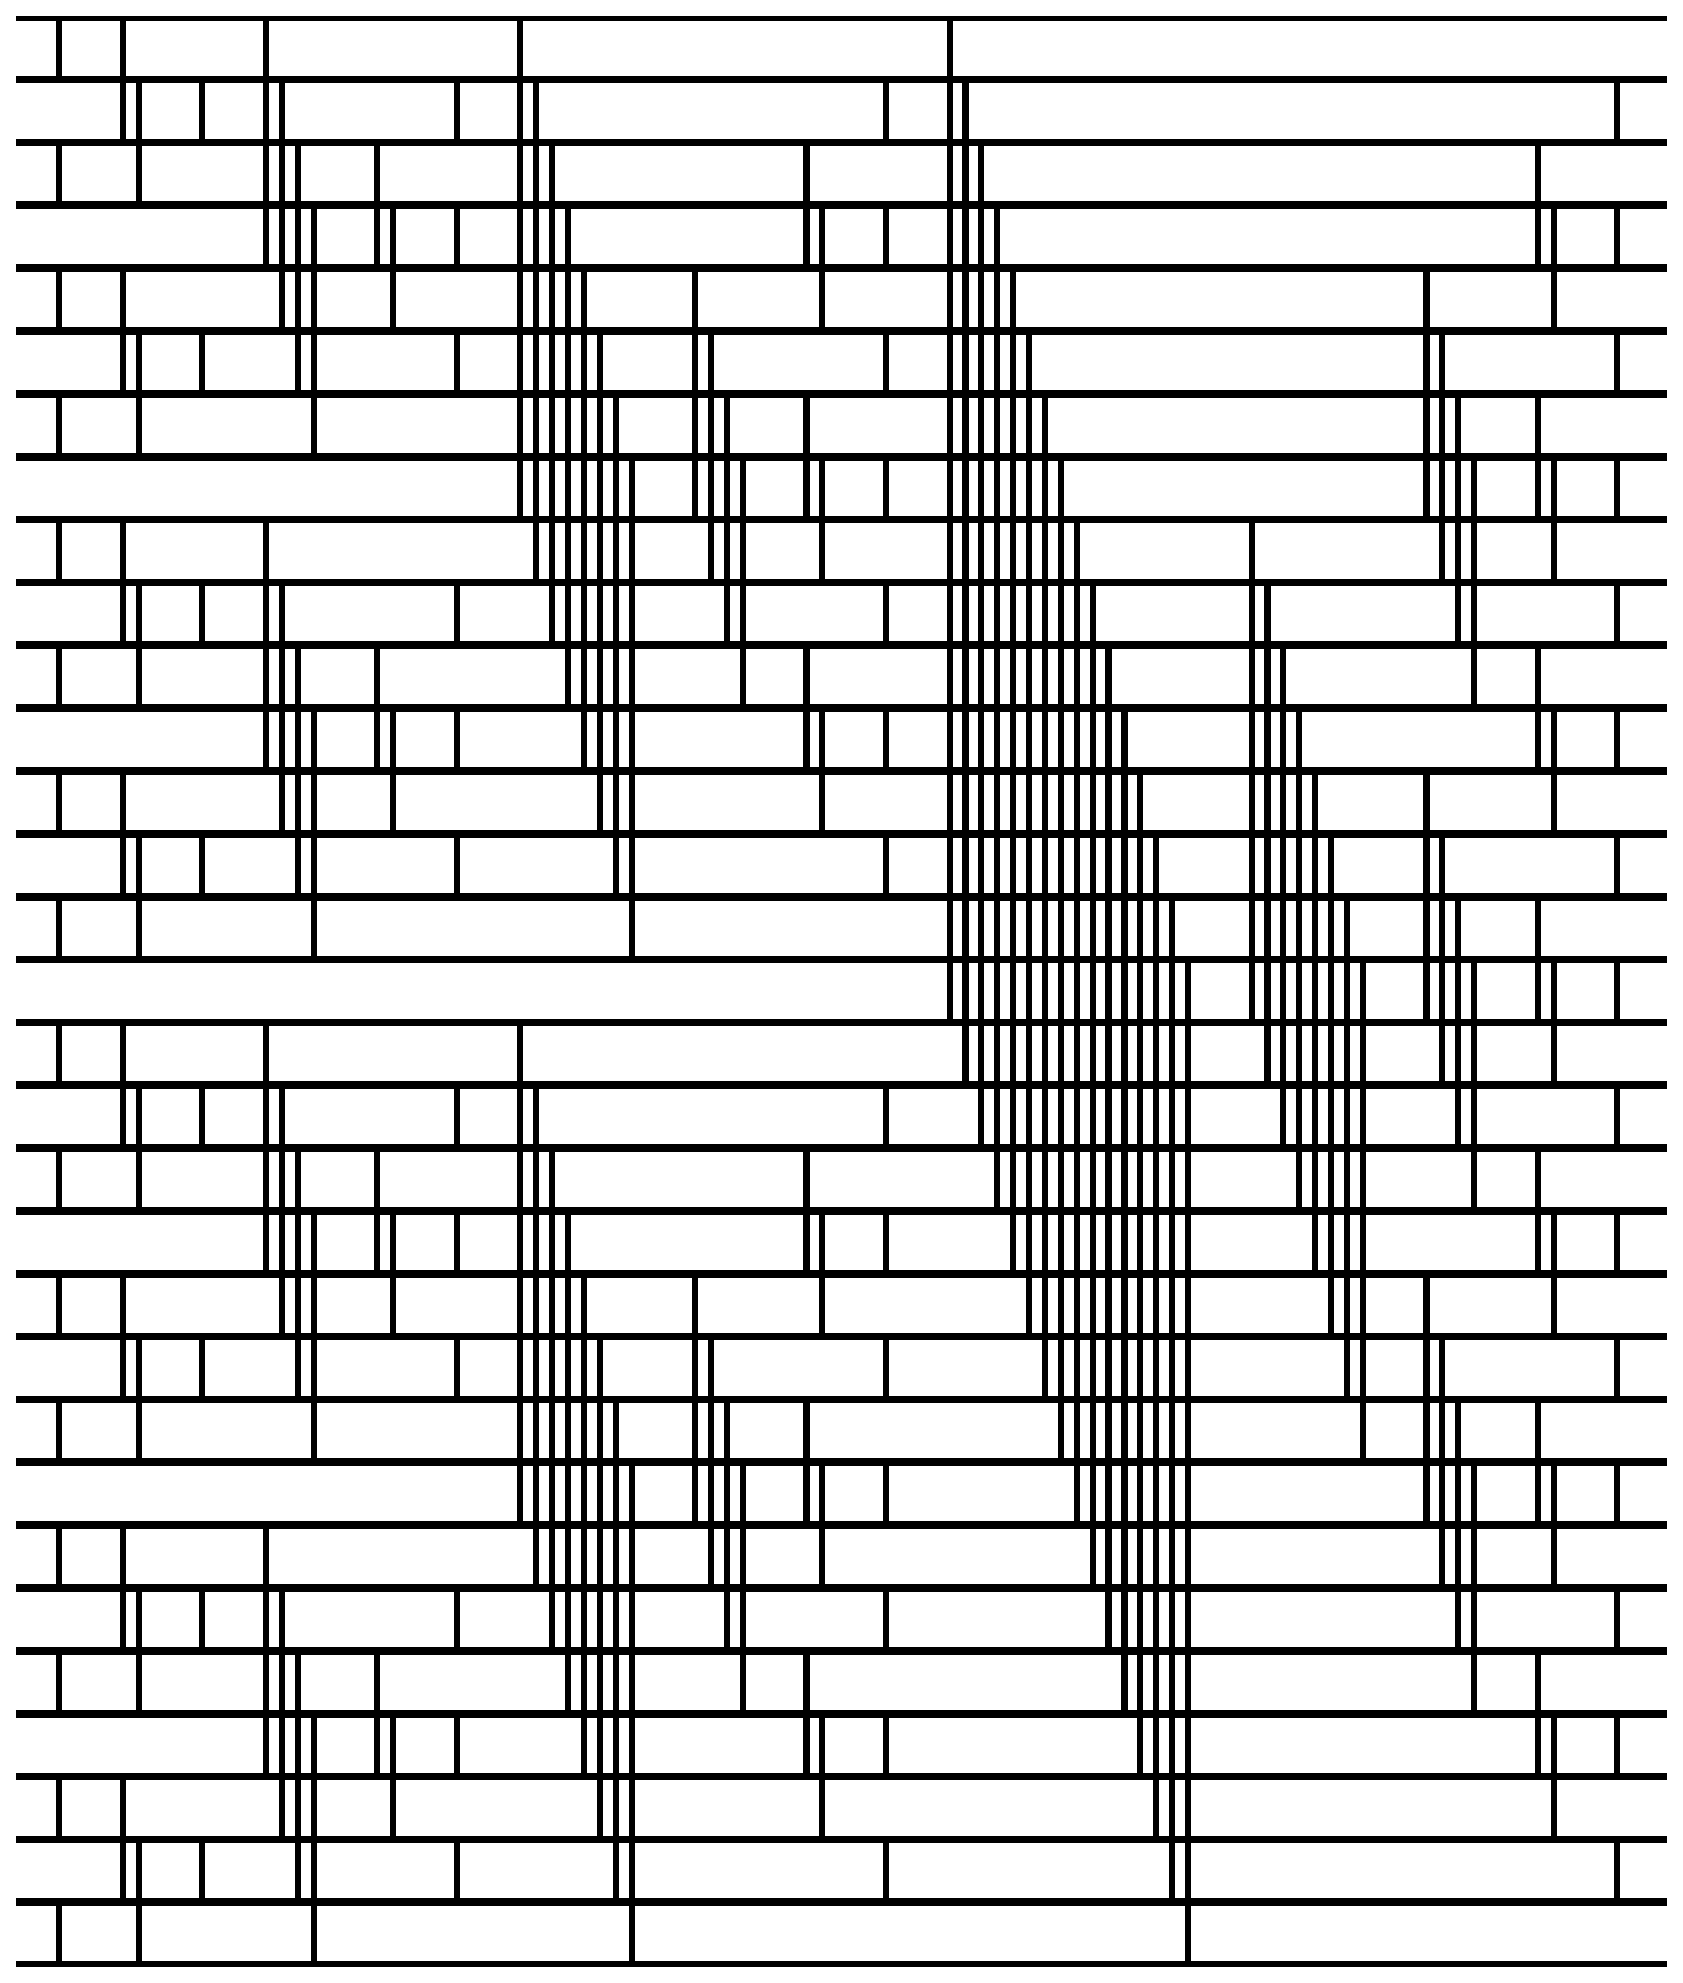
\includegraphics[width=\textwidth]{kep/sort32.eps}
					\caption{$n=32$}
				\end{subfigure}
				\caption{}
				\label{fig:batcher-sort}
			\end{figure}
		A hálózatban a vízszintes vonalak az egyes tárolókat jelölik, amikben a rendeződő értékek vannak, a függőleges vonalak az összehasonlítás és csere műveleteket, ami után az összekötött két elem rendezve van. Egy ilyen pár rendezése után vagy a felső a nagyobb, vagy az alsó, minden pár esetén egyformán, hogy konkrétan melyik, az a medián szempontjából mindegy. Az idő ,,jobbra telik''.

		A 25 elem mediánjának kiválasztásához a 32 elemet rendező hálózatból indultam ki. Ebből kitöröltem azokat az összehasonlításokat, amelyekre nincs szükség. Ez az átalakított hálózat \aref{fig:median25}. ábrán látható.
		\begin{figure}[h]
			\centering
			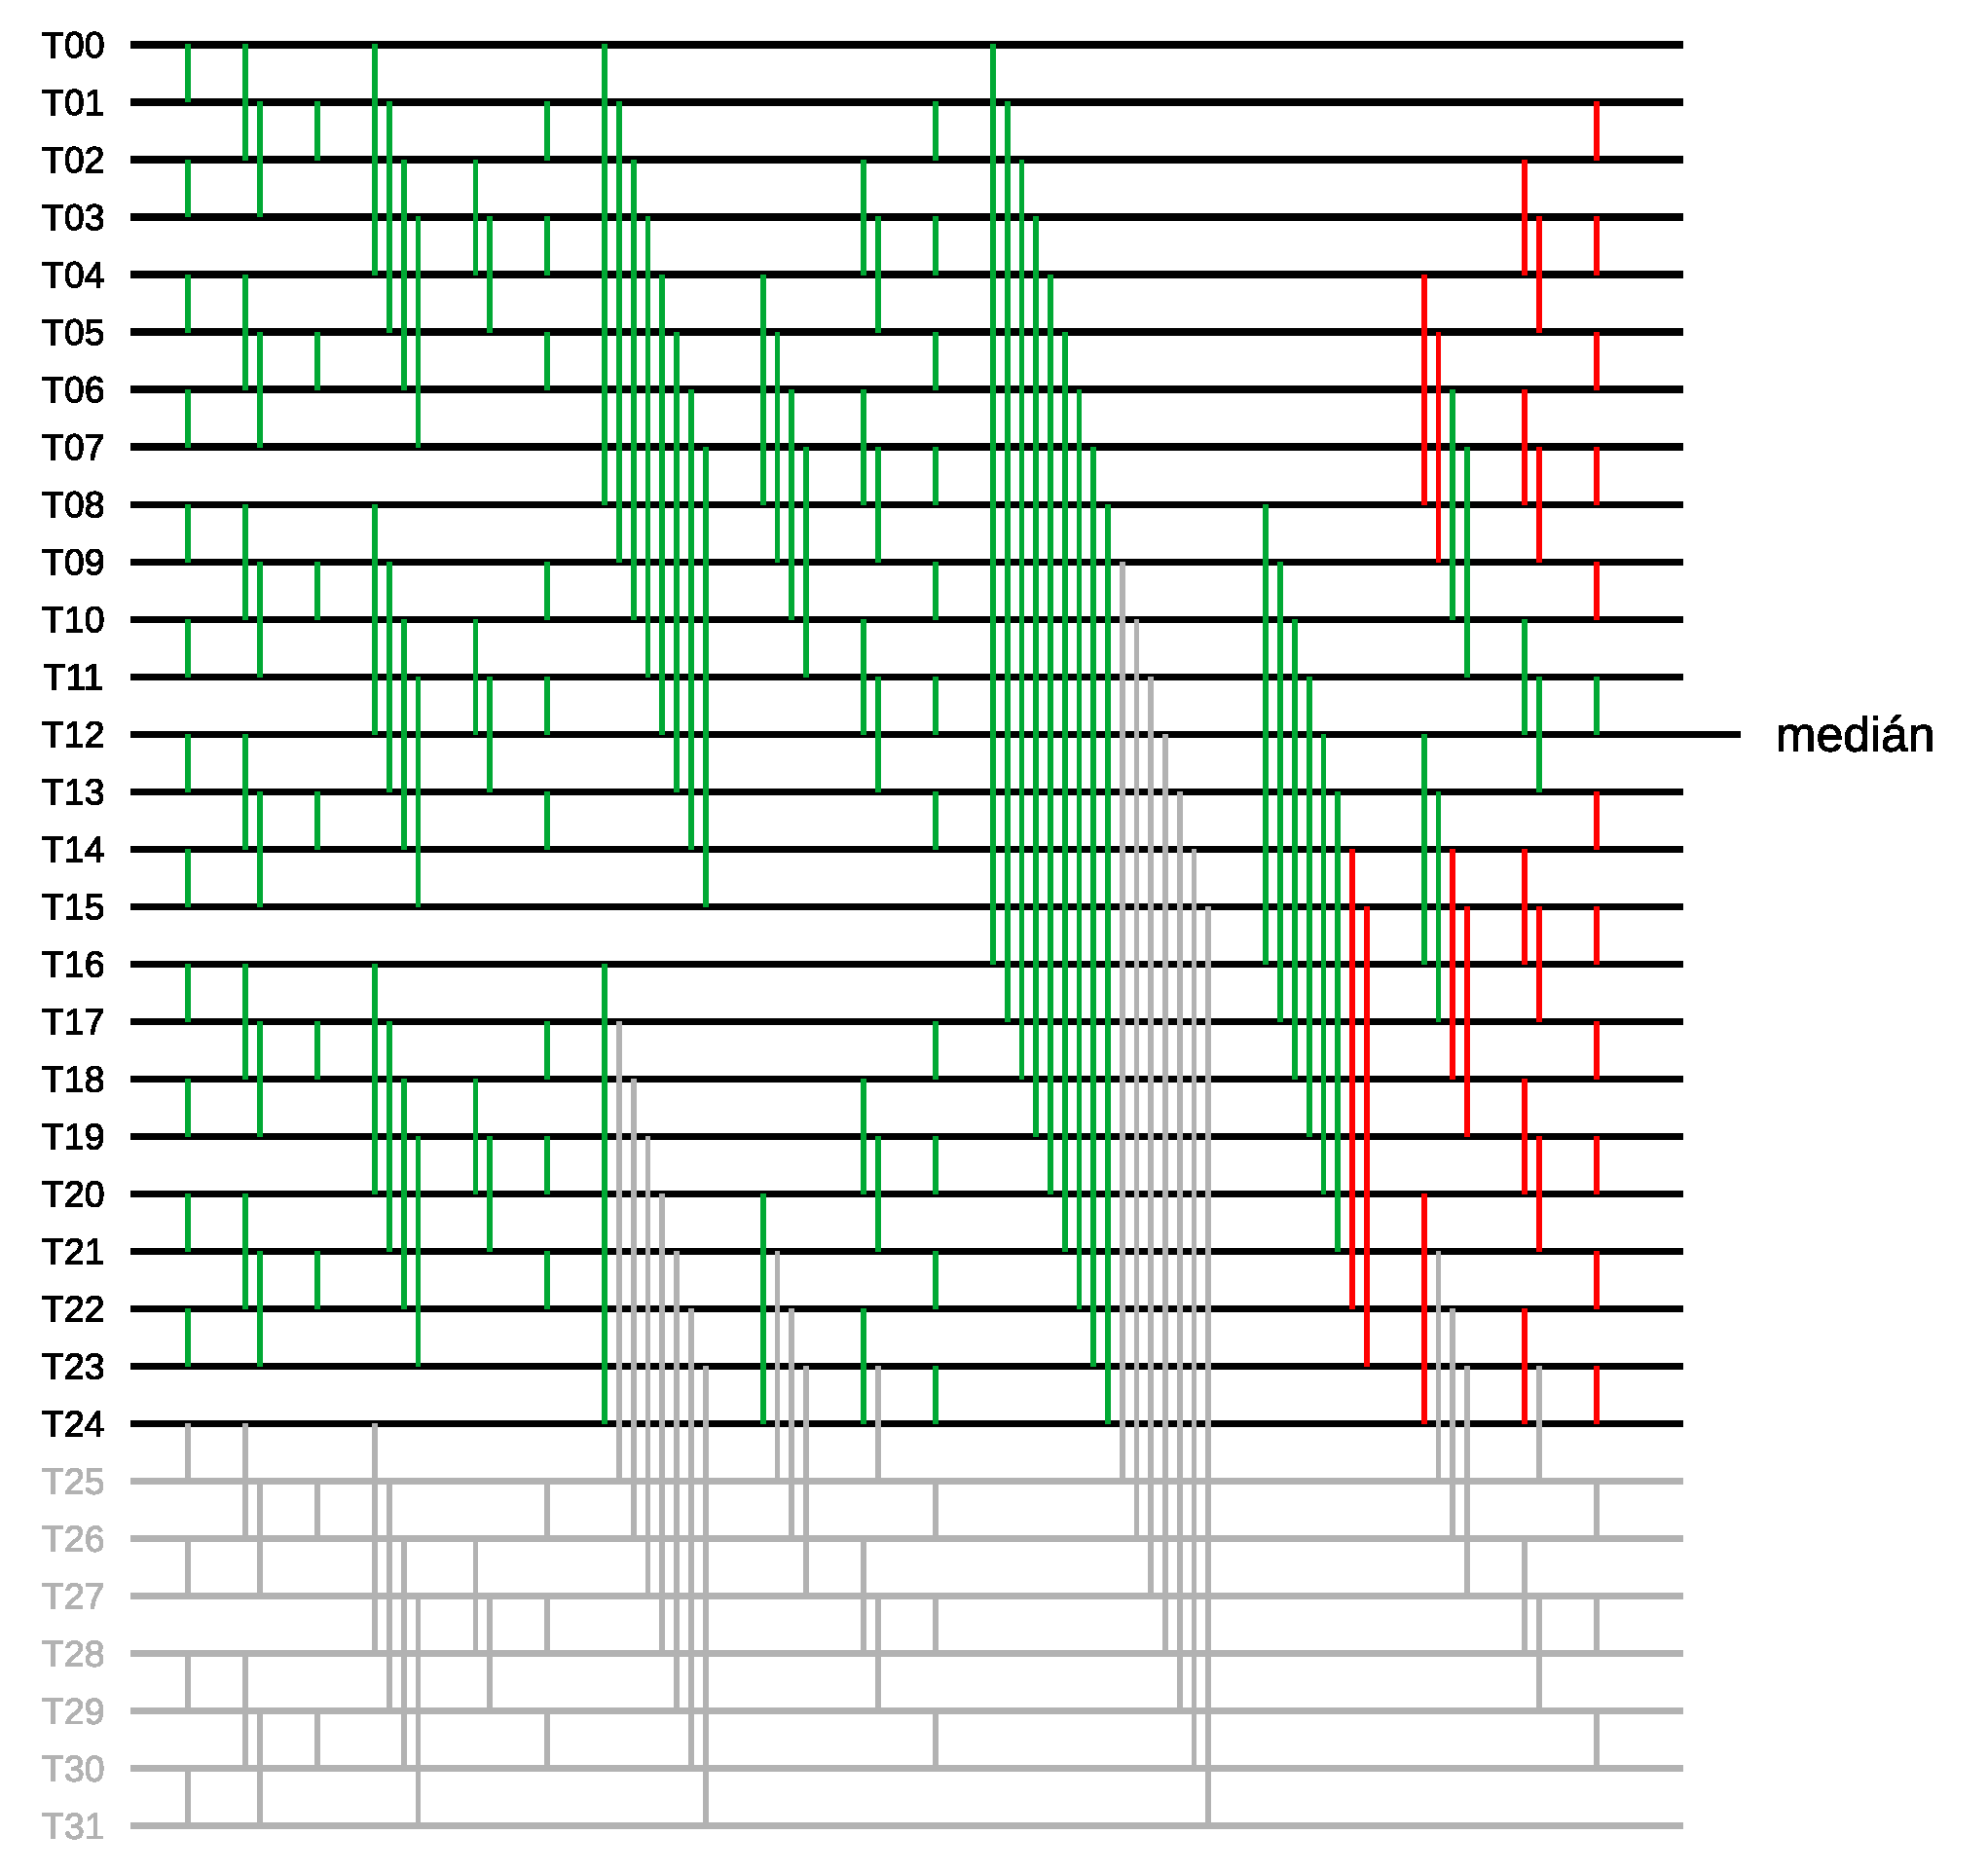
\includegraphics[width=0.8\textwidth]{kep/median25.eps}
			\caption{A 25-ös mediánkiválasztáshoz szükséges hálózat.\\ (zöld: szükséges rendezés, szürke: 32 helyett 25 elem miatt szükségtelen rendezés, piros: teljes rendezés helyett mediánkiválasztás miatt szükségtelen rendezés)}
			\label{fig:median25}
		\end{figure}

		Az $n$ elem rendezéséhez szükséges összehasonlítások sorozata algoritmikusan generálható $n=2^k$-ra \cite{batcher}. Ez alapján írtam egy egyszerű C-programot, ami az összehasonlítássorozat kódját generálja a különböző megoldásokhoz ($m=25$-re), de ez a sorozat még tartalmazza a mediánkiválasztáshoz szükségtelen összehasonlításokat.
		\lstinputlisting{code/avx_omp/comparison_generator.c}

	\section{Sztenderd C implementáció}
		A szűrőprogram első megvalósítása egy egyszerű skalár C program, ami referenciaként szolgál a többi megvalósításhoz, így meg lehet tudni, hogy az egyes hardveres gyorsítási módszerek hogyan teljesítenek. A kép a memóriában egy \verb|char| tömbként van tárolva, három egymásmelletti bájt jelenti egy pixel három színkomponensét.

		Ennél a változatnál nem foglalkoztam az összehasonlítások mediánszámítás miatti lecsökkentésével, csak a 25 db elemen kívüliekre vonatkozókat hagytam el. A fentebb leírt algoritmus szerint generálom futás közben a következőnek rendezendő elempár indexeit. Ezen kívül egyszerűen egyesével végiglépkedek a kép pixelein, ehhez a belső ciklus az $x$ irányú, a külső az $y$ irányú.
		
		A sztenderd C implementáció forráskódja \aref{appendix:avx2_omp} függelékben látható.

	\section{AVX2 + OpenMP implementáció}
		Ehhez a megoldáshoz egyrészt az AVX2 utasításkészlet vektorutasításait használtam fel, másrészt az OpenMP API-t, aminek a segítségével többszálúsítható a képfeldolgozás.
		\subsection{AVX2}
			Az AVX2 utasításkészlet 256 bites vektorutasításokat tartalmaz többféle vektor-adattípusra, többek között 32 db \verb|uint8|-ból, más néven \verb|char|-ból álló vektorra is. Fontos, hogy létezik maximum, és minimumkiválasztó vektorutasítás \verb|uint8| vektorokra, ezek adják az algoritmus lelkét. Két vektorregiszter (\verb|a| és \verb|b|) elemeinek páronkénti rendezése a következő séma szerint történik egy harmadik ideiglenes vektorregiszter (\verb|tmp|) segítségével. Ezután \verb|a| $i$-edik eleme kisebb vagy egyenlő, mint \verb|b| $i$-edik eleme.
			\begin{lstlisting}
	temp = _mm256_max_epu8(a,b);
	a = _mm256_min_epu8(a,b);
	b = temp;\end{lstlisting}

			Az AVX2-es gyorsítás alapgondolata az volt, hogy mindig, amikor a skalár kódban egy bájton dolgozik a program, akkor ehelyett a vektorizált kódban 32 db, egymás melletti bájton dolgozzon párhuzamosan. Ezzel egy mediánkiválasztás végrehajtása gyakorlatilag ugyanúgy zajlik, mint skalár esetben, csak a végén nem egy bájt az eredmény, hanem 32 egymás melletti bájt. Ez a 32 egymás melletti bájt nem feltétlenül pixelhatáron kezdődik vagy végződik, de ez nem okoz gondot, mivel a különböző színcsatornákra teljesen függetlenül kell elvégezni a számítást. A memóriahozzáférés szemléltetéséhez segít \aref{fig:vektorolvasas}. ábra.

			\begin{figure}[h]
				\centering
				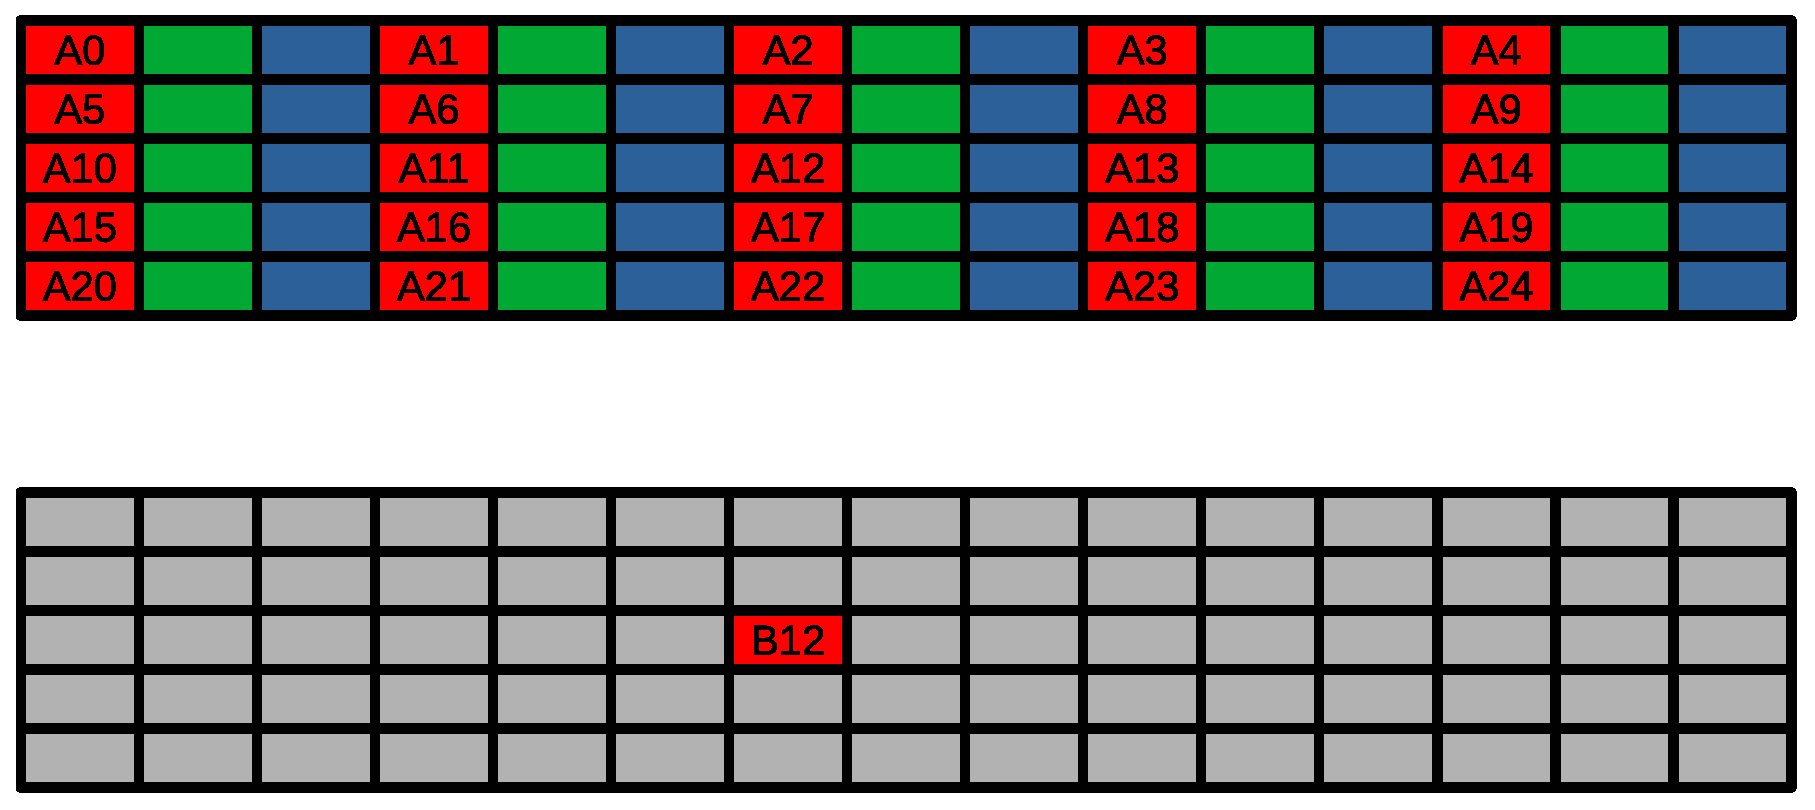
\includegraphics[width=0.8\textwidth]{kep/vektorolvasas.eps}
				\caption{A memóriahozzáférés szemléltetése.}
				\label{fig:vektorolvasas}
			\end{figure}

			\Aref{fig:vektorolvasas}. ábrán az $A_x$-szel jelölt téglalapok azt a 25 címet jelölik a memóriában, ahonnan a bemeneti képből olvasni kell, hogy előállíthassuk a kimeneti kép $B_{12}$ című színkomponensét. Például $A_1=A_0+3$ és $A_5=A_0+3\times W_F$, ahol $W_F$ a kiterjesztett bemeneti kép szélessége pixelben. A skalár kódban ténylegesen ezekről a címekről kellene olvasni egy-egy bájtot, majd a 25 db beolvasott bájt mediánját, ami szintén egy bájt, kellene kiírni a $B_{12}$-es címre. Ehelyett a vektorizált kódban az $A_x$-től az $A_{x}+31$-ig terjedő 32 bájt hosszú tartományt olvasom be és a mediánok vektorát a $B_{12}$-től a $B_{12}+31$-ig terjedő területre írom ki. Ezután a következő olvasássorozatban a bal felső sarokhoz tartozó olvasás a jelenlegi $A_0+32$-es címen fog kezdődni, tehát 32 bájtosával lépegetek. A sorvégekkel nem kell foglalkozni, mert a kimeneti kép szélessége pixelben 32-vel osztható.

			Mivel az AVX2-es utasításkészletet támogató, de AVX-512 nélküli processzorokban csak 16 db vektorregiszter van, ezért nem fér el mind a 25 db beolvasott, plusz a rendezéshez használt ideiglenes tároló vektorváltozó regiszterekben, így a medián keresése során bizonyos változókat ideiglenesen ki kell írni memóriába majd visszaolvasni. Ez a kiírás-visszaolvasás akkor is megtörténne, ha csak rábíznám a fordítóra, de valamit lehet javítani a futási időn, ha a saját kezembe veszem a dolgot és explicit módon leírom a kódba, hogy mikor melyik regiszterben melyik vltozó legyen és mikor történjenek a kiírások és a visszaolvasások, mert így csökkenthető a memóriahozzáférések száma. Ezzel az is együtt jár, hogy gyakorlatilag kézzel unrollolnom kell az összehasonlítások sorozatát generáló kódrészt és még ezt is meg kell variálnom a vektorregiszterek kezelése miatt. Ennek az unrollolásnak az a nagy előnye, hogy az összehasonlítandó változók indexeinek kiszámításának overheadje teljesen megszűnik és a mediánkiválasztás közben nincs elágazás a kódban, ami elég hatékony végrehajtást tesz lehetővé. A vektorregiszterek menedzselését \aref{fig:vektorregiszterek}. ábra szemlélteti.

			\begin{figure}[h]
				\centering
				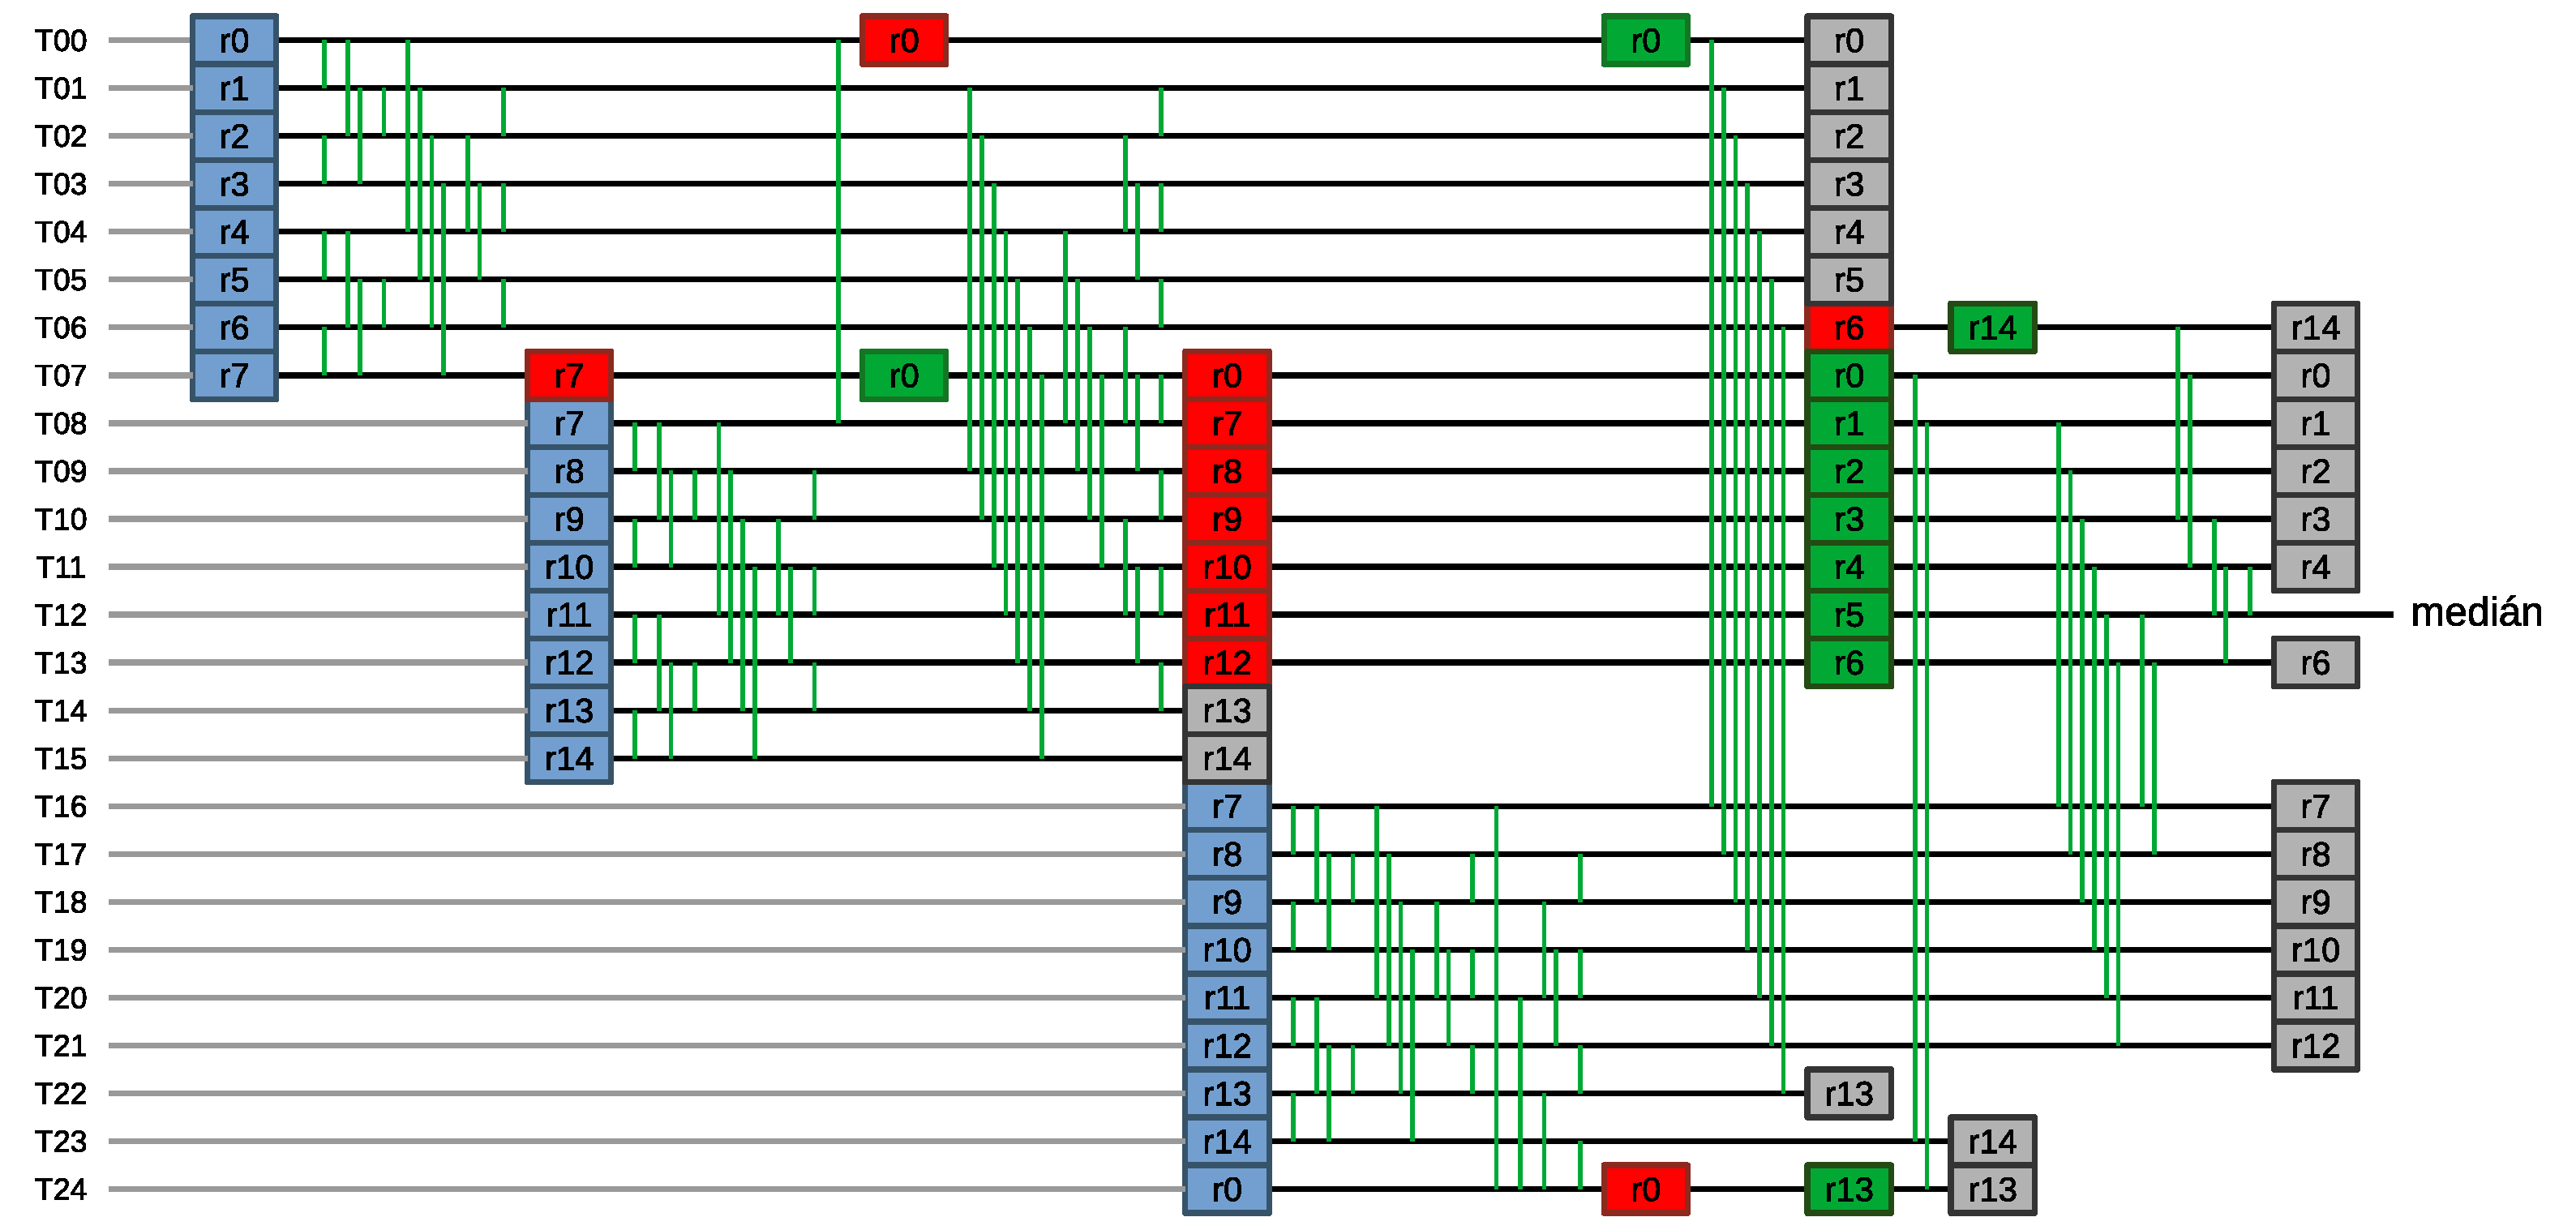
\includegraphics[width=\textwidth]{kep/vektorregiszterek.eps}
				\caption{A vektorregiszterek menedzselése.}
				\label{fig:vektorregiszterek}
			\end{figure}

			\Aref{fig:vektorregiszterek}. ábrán $T_{XX}$ és a mellette lévő vízszintes vonal jelöli az egyes vektorváltozókat, a függőleges zöld vonalak pedig a rendezéseket két ilyen változó között. A kódban az egyes regiszterek szigorúan véve egy-egy változóként vannak deklarálva, de itt változó alatt azokat az adatvektorokat értem, amik közben néha ki is íródnak a memóriába és az elemeik össze-vissza cserélődnek, de magát az adatvektort végig számon kell tartani. A kék téglalap, benne egy regiszter nevével ($r_{XX}$) azt jelenti, hogy akkor olvassom be a bemeneti képből az adott vektorváltozót, ami egy unaligned load utasítást jelent. A piros téglalap benne egy regiszter nevével azt jelenti, hogy a regiszter tartalmát (ami az aktuális vízszintes vonalhoz tartozó változó) kiírom egy kis ideiglenes tároló tömbbe egy aligned store utasítás segítségével, hogy ez a regiszter használható legyen egy másik változó tárolására. A szürke téglalap hasonló dolgot jelent, mint a piros, ez is az adott regiszter felszabadulását jelenti, azzal a különbséggel, hogy itt nincs szükség store utasítással kiírni az ideiglenes tömbbe az adott $r_{XX}$ regiszter tartalmát, mert az aktuálisan benne tárolt változóra innentől már nincs szükség, egyszerűen felülírható egy másik változóval. Végül pedig a zöld téglalap, ami a piros párja, az aligned load utasítást jelenti, amikor az aktuális vízszintes vonalnak megfelelő változót beolvasom a zöld téglalapban megjelölt $r_{XX}$ regiszterbe. Logikus, hogy minden piros store után ugyanabban a sorban van egy zöld load, hiszen eleve azért írom ki a változót, hogy később visszaolvasva még használjam.

			Összesen egy mediánvektor (32 bájt) kiszámolásához 25 db unaligned loadra (kék), 11 db aligned store-ra (piros), 11 db aligned loadra (zöld) és 1 db unaligned store-ra van szükség. És emellett természetesen 113 db páronkénti rendezésre a vektorváltozók között.


			A vektorutasításokat az Intel intrinsic függvényeken keresztül tudom használni. A kódomban a következő intrinsic-eket használtam vagy próbáltam ki \cite{intrinsics}.

			\begin{lstlisting}
_mm256_max_epu8(a, b)					// maximum selection
_mm256_min_epu8(a, b)					// minimum selection
_mm256_lddqu_si256(addr)			// unaligned load
_mm256_storeu_si256(addr, a)	// unaligned store
_mm256_load_si256(addr)				// aligned load
_mm256_store_si256(addr, a)		// aligned store
_mm_malloc(size, align)				// aligned malloc
_mm_free(addr)								// aligned free
_mm256_stream_si256(addr, a)	// aligned store to RAM, bypassing cache
_mm_prefetch(addr, i)					// prefetch cache line containing addr
	// prefetch into non-temporal cache: i = _MM_HINT_NTA\end{lstlisting}

			Az aktuális mediánszámításhoz szükséges cache line-okat az algoritmus elkezdése előtt prefetch-elem, hogy potenciálisan kevesebb időt kelljen várni a loadokra a számolás közben. Ennek a változtatásnak tapasztalatom szerint nagyon kicsi, de pozitív hatása van. Kipróbáltam különböző prefetch módokat is (az \verb|i| változó értéke), minimális különbséget tapasztaltam, a fent látható non-temporal cache-be való olvasás nyert. Ahol lehet, ott unaligned load helyett aligned load-ot használok a kódban, de tapasztalatom szerint ennek is csak minimális hatása van a futási időre. Az egyik leginkább kritikus pontja a programnak a kiszámolt mediánok kirása a memóriába. Itt ismert, hogy mindig 32 bájtra aligned címre kell írni, így használható valamilyen aligned store. A \verb|_mm256_stream_si256()| és \verb|_mm256_store_si256| intrinsic-ek közül az előbbit, a cache-t kikerülő verziót találtam kicsivel gyorsabbnak.
		\subsection{OpenMP}
			Az algoritmus többszálúsítása már valamivel egyszerűbb az OpenMP pragmakészlet segítségével. A kód párhuzamosítással foglalkozó része a következő.
			\begin{lstlisting}
register __m256i r00, r01, r02, r03, r04, r05, r06, r07,\
				 r08, r09, r10, r11, r12, r13, r14, tmp;
int y_out, x_rgb_out;

#pragma omp parallel private( y_out, x_rgb_out, \
	r00, r01, r02, r03, r04, r05, r06, r07, r08, r09, r10, r11, r12, r13, r14, tmp) \
	shared(imgHeight, imgWidth, imgWidthF, imgSrcExt, imgDst)
{
	// array to temporarily store register contents when registers need to be freed
	__m256i* arr = (__m256i*)_mm_malloc(25 * 32, 32);

#pragma omp for schedule(dynamic)
	for (y_out = 0; y_out < imgHeight; y_out++)
	{
		for (x_rgb_out = 0; x_rgb_out < imgWidth * 3; x_rgb_out += 32)
		{
			// calculate median
			// store median to output
		}
	}
	_mm_free(arr);
}\end{lstlisting}

			A fenti kódrészletben az első \verb|#pragma| a párhuzamos rész kezdete, itt explicite megadom a változókról, hogy melyik shared és melyik private. A képen belüli ,,navigáláshoz'' használt ciklusváltozókból minden szálnak sajátra van szüksége, mert ezzel indexelik azt a részt a bemeneti és kimeneti memóriaterületeken ahol éppen számolnak. Vektorregiszterekből (\verb|r00| - \verb|r14|, \verb|tmp|) minden szálnak saját példányokra van szüksége, mert független számításokat végeznek más-más adatokon, így ezek is privátok lesznek. A bemeneti és kimeneti kép címei és méretei pedig jó, ha shared változók, mert ezeket csak olvassák az egyes szálak és a bennük tárolt információkra mindegyiknek szüksége van. Elvileg lehetne probléma abból, hogy több szál akar ugyanonnan olvasni, de hamar minden szál becache-eli ezt a néhány adatot magának, így nem interferálnak egymással az olvasások során. Annyit még megjegyzek, hogy az \verb|arr| ideiglenes tömb lefoglalása és felszabadítása is a párhuzamos blokkon belül zajlik, tehát ebből a tömbből is minden szálnak saját, független példánya van.

			A következő \verb|#pragma| a külső, kép sorain iteráló ciklusra vonatkozik, annak az iterációit osztja fel a szálak között. A \verb|schedule(dynamic)| pragma a ciklus iterációinak szálak közötti szétosztását vezérli. Gyakorlatilag $n$ db szál és $H$ sorból álló kép esetén minden szálnak egy folytonos, $\lceil H/n\rceil$ sorból álló sáv jut a képből. Ezáltal minimális lesz azoknak a memóriaterületeknek a mérete két ilyen sáv határánál (határonként 4 sor), amelyeket a bemeneti képből mindkét szál olvas valamikor, így esélye van az ütközésnek. Egyébként az ütközés gyakorlatilag kizárt, mert amennyire értem, a saját sávjukon belül minden szál fentről lefelé halad, így amikor egy határvonal fölött dolgozó szál a határ közelébe ér, a határvonal alatt dolgozó szál már régen eltávolodott onnan.
			
			Kipróbáltam azt is, amikor az egy soron belüli iterálásra vonatkozik a párhuzamosítás és egyben ez a külső ciklus, így körülbelül 30\%-kal romlott a program teljesítménye, így az előző verziónál maradtam. Azért lehet jogos, hogy romlik a teljesítmény, ha függőleges sávokra osztom a képet, mert amikor egy szál már végigért a sávja egy során és éppen kezdi a következőt, de a tőle balra lévő sávhoz tartozó szál még éppen a sora végén jár, akkor  átlapolódás van a két szál által olvasott memóriaterületek között. Ennek fényében nem gondolom, hogy ennek a problémának 30\%-os sebességromlást kellene okoznia.

			Az AVX2 + OpenMP implementáció forráskódja \aref{appendix:avx2_omp}. függelékben látható.


	\clearpage
	\section{OpenCL implementáció}
		Az OpenCL verzió half precision float (\verb|half|) típust használ, mert a teszteléshez használt GPU is és az osztályozáshoz használt GPU is ilyen típussal tud a leggyorsabban számolni. Az előbbi a teszteléshez használt processzorba integrált GPU (Intel UHD Graphics for 11th Generation Intel Processors, UHD 730 \cite{intel-opt-guide}), az utóbbi pedig egy NVIDIA TITAN Xp videókártya lesz, ha minden igaz (Pascal architektúra, \cite{pascal}). Ezen kívül az is szempont volt a \verb|half| típus használatánál, hogy viszonylag kis fejfájással és kicsivel több shared memória felhasználásával meg lehet oldani, hogy elvben ne történjen bankütközés a shared memória olvasásakor.

		A számítás menete a gyakorlaton megismerttel gyakorlatilag megegyezik. Először a thread block (workgroup) szálai bemásolják a globális memóriából a szükséges részt a shared (local) memóriába, közben átkonvertálják a beolvasott \verb|char| értékeket \verb|half| típusra, a shared memóriában már így tárolódik a beolvasott adat. Ezután bevárják egymást, majd minden szál a saját regisztereibe olvas 25 db \verb|half| értéket a shared memóriából, ezeken megkeresi a mediánt, majd az eredményt visszakonvertálja \verb|char| típusra és kiírja a globális memóriába. Ezt a shared memória feltöltés utáni részt minden szál a hozzá tartozó pixel 3 színcsatornájára végzi el egymás után, vagyis szálanként 3 bájtnyi kimenet keletkezik.
		
		A bankütközés elkerülése \verb|half| adattípusok esetén a következőképpen történik. Ha egyszerűen egy háromdimenziós \verb|half| tömböt deklarálok a következőképpen, akkor \aref{fig:gpu_bank_collision_f16_16}. ábrán látható módon lesznek ütközések. (Az ábrákon a sorokat félbe törtem, hogy olvasható legyen. A szürkített részeknél kell összeragasztani a félsorokat.)
		\begin{lstlisting}
__local shmem[20][20][3];\end{lstlisting}
		
		\begin{figure}[h]
			\centering
			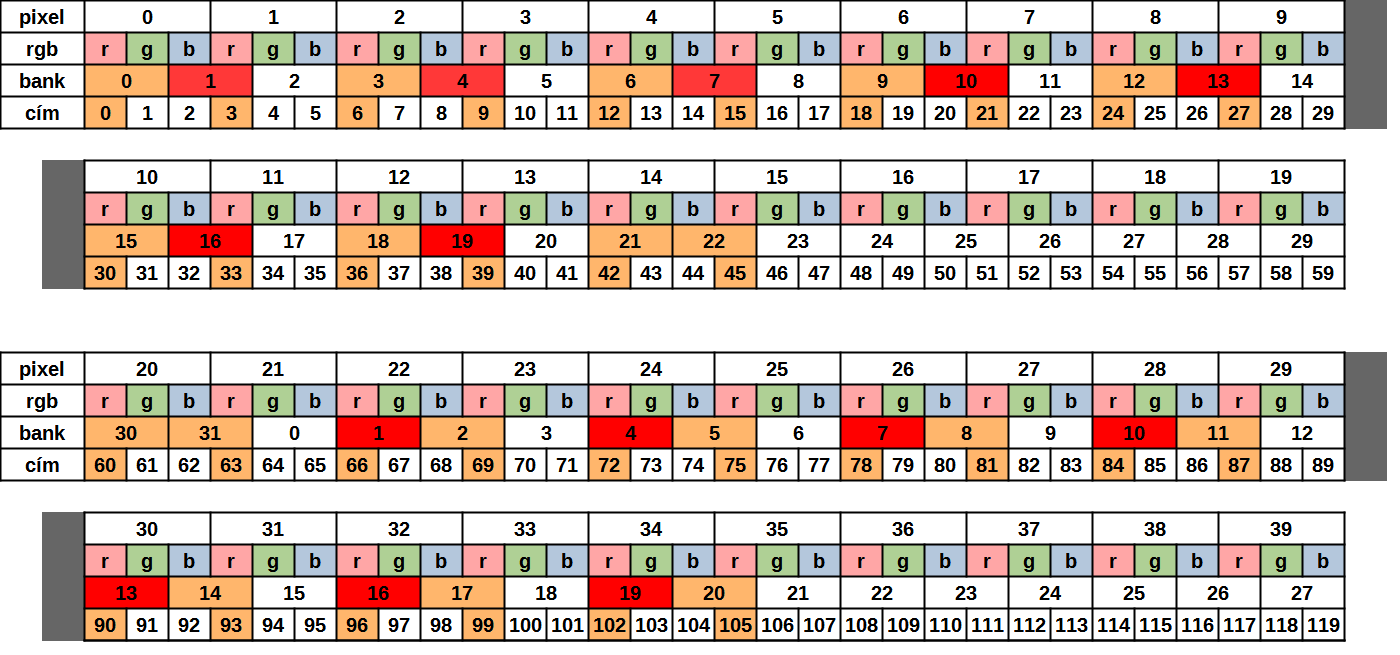
\includegraphics[width=\textwidth]{kep/gpu_bank_collision_f16_16.png}
			\caption{Banütközések $16\times16$-os blokkméretnél, half precision float típussal.}
			\label{fig:gpu_bank_collision_f16_16}
		\end{figure}
		\Aref{fig:gpu_bank_collision_f16_16}. ábrán a ,,pixel'' sor jelenti az adott pixel lineáris sorszámát a thread block bemeneti régióján belül. Az ,,rgb'' sorban az adott pixelek színkomponensei vannak felsorolva. A ,,bank'' sorban az látszik, hogy a fölötte lévő színkomponens melyik bankba esik a shared memóriában. A ,,cím'' sorban pedig a shared memóriában lévő tömbön belüli lineáris cím van, ahol az adott komponens található. Narancssárga jelöli azokat a címeket és a hozzájuk tartozó bankokat, amikről először olvasnak egy warp szálai (32 db). Pirossal pedig azokat a bankokat jelöltem, amiknek az elérésekor bankütközés történik.
		
		A fenti alapértelmezett elrendezésnél kb. minden második olvasás jár bankütközéssel, ami nem tragikus, de a bankütközéseket el lehet kerülni teljesen. Az sem sokat javít a helyzeten, ha $32\times8$-asra változtatom a blokkméretet, ennek a hatása \aref{fig:gpu_bank_collision_f16_32}. ábrán látható.
		
		\begin{figure}[h]
			\centering
			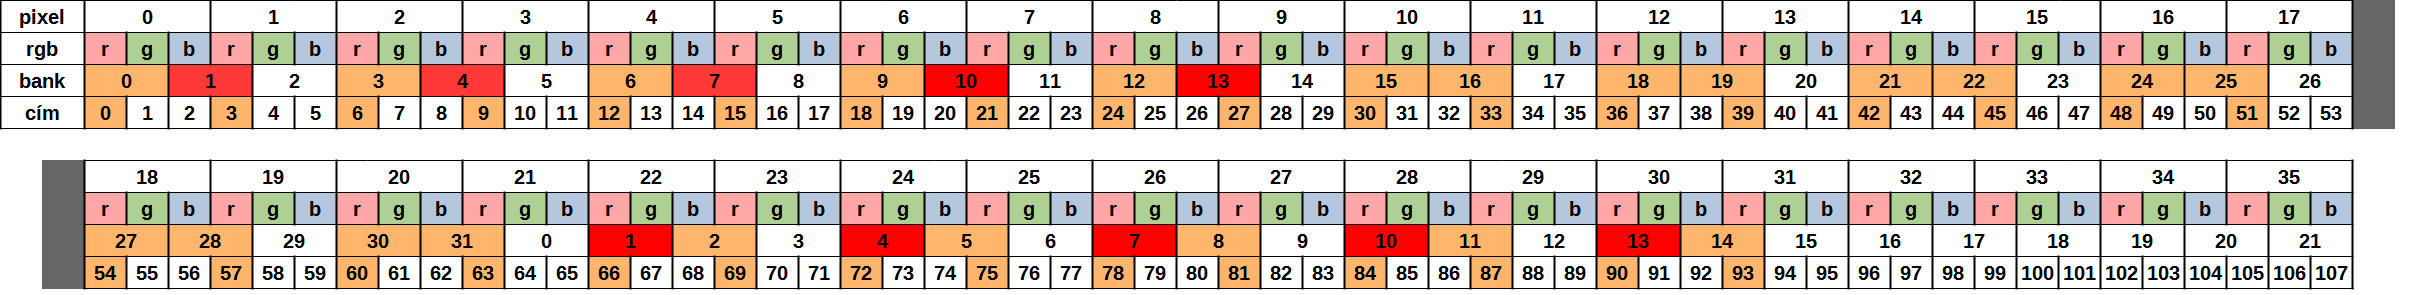
\includegraphics[width=\textwidth]{kep/gpu_bank_collision_f16_32.png}
			\caption{Banütközések $32\times8$-as blokkméretnél, half precision float típussal.}
			\label{fig:gpu_bank_collision_f16_32}
		\end{figure}
		Végül az jelenti a megoldást, ha maradok a $16\times16$-os blokkméretnél és a shared memória deklarációját a következőre cserélem.
		\begin{lstlisting}
__local half shmem[20*4+2][20];\end{lstlisting}
		Ez azt jelenti, hogy bemeneti pixelenként nem három, hanem négy színcsatornányi hellyel számolok (a negyediket nem használom) és még a sorok végén két \verb|half|-nyi, ezzel éppen egy banknyi üres helyet hagyok. Ezzel azt érem el, hogy a párhuzamos olvasásoknál minden második bank van használatban, tehát az első sorban a páros indexűek, a második sorban ugyanilyen séma szerint éppen a páratlan indexűek lesznek használatban, így nincs bankütközés. Ez a változat \aref{fig:gpu_bank_collision_f16_16_rgbx_padded}. ábrán látható.
		
		\begin{figure}[h]
			\centering
			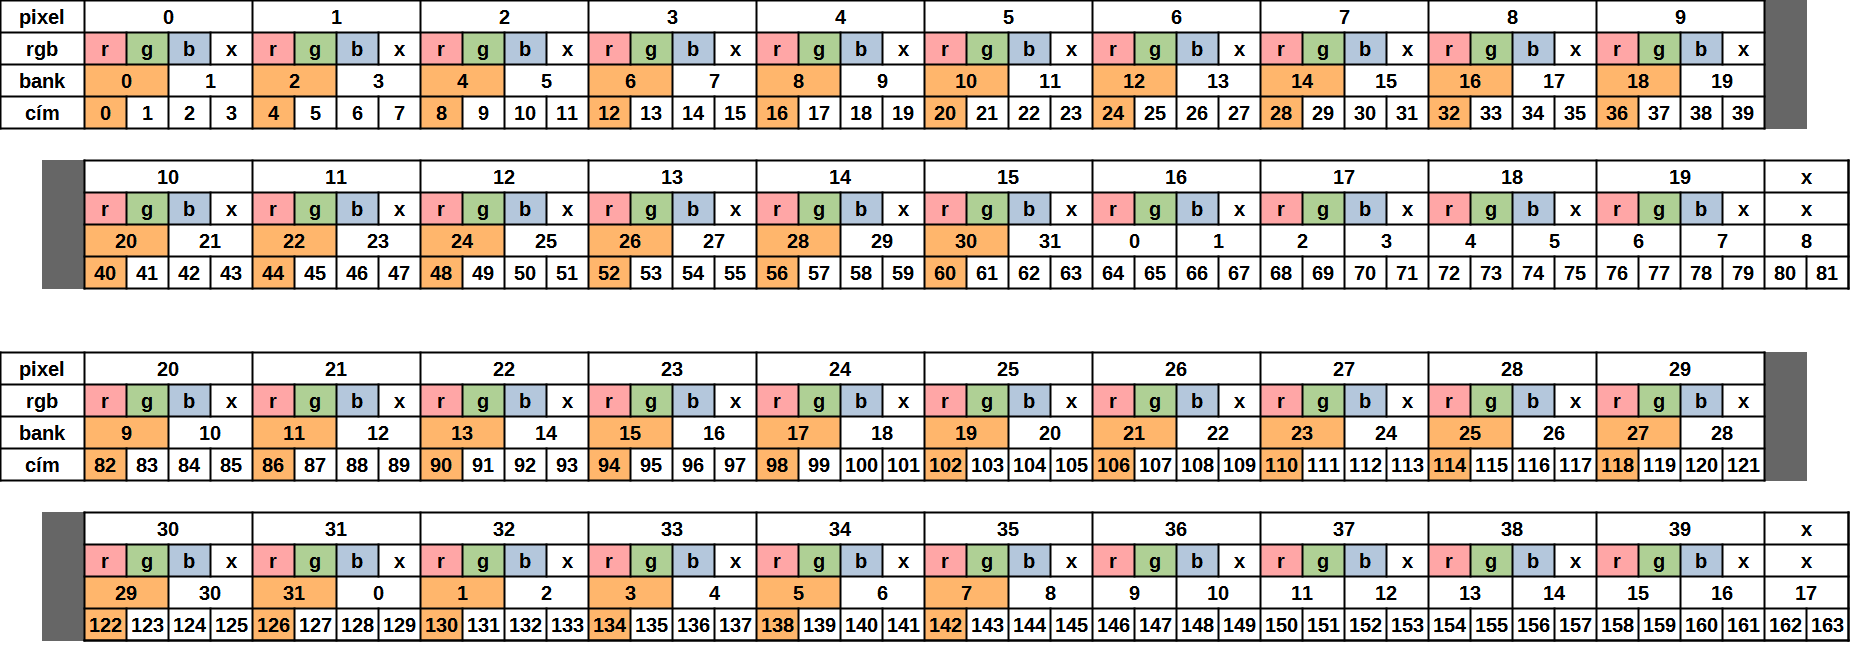
\includegraphics[width=\textwidth]{kep/gpu_bank_collision_f16_16_rgbx_padded.png}
			\caption{Nincs bankütközés $16\times16$-as blokkméretnél, half precision float típussal, negyedik virtuális színcsatornával és sorvégi offsettel.}
			\label{fig:gpu_bank_collision_f16_16_rgbx_padded}
		\end{figure}
		A negyedik virtuális színcsatorna vagy a sorvégi offset magában nem elég a bankütközések elkerülésére, $16\times16$-os és $32\times32$-es blokkméretek mellett sem.
		
		A fenti shared memória deklarációval a következőképpen módosul a shared memória indexelése az eredeti, háromdimenziósnak deklarált tömbhöz képest.
		\begin{lstlisting}
shmem[x][y][rgb] -> shmem[x*4+rgb][y]\end{lstlisting}

			Az OpenCL implementáció forráskódja \aref{appendix:ocl_kernel}. függelékben látható.


\clearpage
	\section{Futási idők}
		A teszteléshez használt hardver egy Intel i5-11400 processzor fix \qty{2600}{MHz}-es órajellel, \qty{3200}{MHz}-es DDR4 RAM-mal. A használt GPU ugyanennek a processzornak az integrált GPU-ja, ami ugyanezt a RAM-ot használja (Intel UHD 730 Graphics \cite{intel-opt-guide}).\\[3ex]
		\begin{tabular}{|l||r|r|r|}
			\hline
			Implementáció & Futások száma & Egy futás átlagos ideje & MP/s\\
			\hline
			\hline
			C & 10 & \qty{90430.6000}{ms} & \qty{0.2067}{}\\
			\hline
			AVX2 + OpenMP referencia & 1000 & \qty{13.6100}{ms} & \qty{1373.2585}{} \\
			\hline
			AVX2 + OpenMP & 1000 & \qty{13.2500}{ms} & \qty{1410.5697}{} \\
			\hline
			OpenCL referencia & 100 & \qty{69.8705}{ms} & \qty{267.4954}{} \\
			\hline
			OpenCL & 500 & \qty{42.8274}{ms} & \qty{436.4044}{} \\
			\hline
		\end{tabular}

	\clearpage
	\bibliographystyle{plain}
	\bibliography{mybib}
	
	\appendix
	\clearpage
	\section{Sztenderd C implementáció kódja}
		(Ez a változat ugyanazokat az egyéb fájlokat használja, mint az AVX2+OpenMP implementáció, csak másik függvény hívódik meg a main-ben.)
		\subsection{median\_filter.cpp}
			\label{appendix:skalar}
			\lstinputlisting{code/skalar/median_filter.cpp}
	\clearpage
	\section{AVX2 + OpenMP implementáció kódja}
		\subsection{defs.h}
			\lstinputlisting{code/avx_omp/defs.h}
		\subsection{func.h}
			\lstinputlisting{code/avx_omp/func.h}
		\subsection{main.cpp}
			\lstinputlisting{code/avx_omp/main.cpp}
		\subsection{median\_filter\_avx\_omp.cpp}
			\label{appendix:avx2_omp}
			\lstinputlisting{code/avx_omp/median_filter_avx_omp.cpp}
	\clearpage
	\section{OpenCL implementáció kódja}
		\subsection{defs.h}
			\lstinputlisting{code/opencl/defs.h}
		\subsection{func.h}
			\lstinputlisting{code/opencl/func.h}
		\subsection{main.cpp}
			\lstinputlisting{code/opencl/main.cpp}
		\subsection{opencl\_kernels.cl}
			\label{appendix:ocl_kernel}
			\lstinputlisting{code/opencl/opencl_kernels.cl}
		\subsection{median\_filter\_ocl.cpp}
			(Ebben a fájlban lévő kernel string literál effektíve ugyanaz, mint a fönti .cl kernel kód.)
			\lstinputlisting{code/opencl/median_filter_ocl.cpp}
		
\end{document}

